\chapter{Vertex cover problem} % Main chapter title

\label{Chapter2} % Change X to a consecutive number; for referencing this chapter elsewhere, use \ref{ChapterX}
\justify
To vertex cover ενός γράφου είναι ένα σύνολο κόμβων τέτοιο ώστε κάθε ακμή του γράφου είναι προσκείμενη σε τουλάχιστον ένα κόμβο του συνόλου αυτού. Το πρόβλημα εύρεσης του ελάχιστου vertex cover είναι κλασικό πρόβλημα στον τομέα της συνδυαστικής βελτιστοποίησης και της θεωρίας υπολογιστών και κλασικό παράδειγμα NP-hard προβλήματος βελτιστοποίησης. 
%----------------------------------------------------------------------------------------
%	SECTION 1
%----------------------------------------------------------------------------------------

\section{Διατύπωση}
Το vertex cover $V'$ ενός μη κατευθυντικού γράφου $G=(V,E)$ είναι ένα υποσύνολο του $V$ τέτοιο ώστε:
$$\forall uv \in{E} \Rightarrow u \in{V'} \lor v \in{V'}$$
Ένα τέτοιο σύνολο λέμε ό τι καλύπτει τις ακμές του $G$. Το ελάχιστο vertex cover ενός γράφου $G$ είναι το σύνολο $V'$ με τον μικρότερο αριθμό στοιχείων.


\begin{figure}[H]
\caption{Vertex cover}
\centering
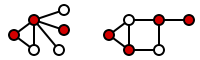
\includegraphics{Figures/vert_cover.png}\centering
\end{figure}

\begin{figure}[H]
\caption{Minimum vertex cover}
\centering
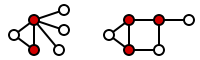
\includegraphics{Figures/min_vert_cover.png}\centering
\end{figure}

%----------------------------------------------------------------------------------------
%	SECTION 2
%----------------------------------------------------------------------------------------

\section{NP-πληρότητα}

Στη γενική περίπτωση το πρόβλημα vertex cover είναι NP-πλήρης οπότε είναι απίθανο να βρεθεί ακριβής αλγοριθμική λύση σε πολυωνυμικό χρόνο εκτός και αν P = NP. H NP-πληρότητα μπορεί να αποδειχθεί με υπαγωγή από το 3-SAT πρόβλημα ή από το Clique πρόβλημα. Σε ειδικές περιπτώσεις γράφων όμως μπορούν να βρεθούν πολυωνυμικοί αλγόριθμοι. Με εξαντλητική αναζήτηση το πρόβλημα μπορεί να λυθεί σε $2^{k}n^{O(1)}$ χρόνο, όπου k το μέγεθος του συνόλου και n ο αριθμός των κόμβων, το οποίο κάνει το πρόβλημα fixed-parameter tractable. Οπότε αν ενδιαφερόμαστε για μικρά k μπορούμε να επιλέξουμε αυτή τη μέθοδο και να έχουμε λύση σε πολυωνυμικό χρόνο.

\section{Λύσεις}

\subsection{Πρόβλημα ακέραιου προγραμματισμού}

Το minimum vertex cover problem μπορεί να διατυπωθεί ως το ακόλουθο πρόβλημα ακέραιου προγραμματισμού

$$min\{\displaystyle\sum_{u\in{V}} c(v)x_v\}$$ 
\centerline{subject to}
$$x_u + x_v \geq{1}, \quad \forall (u, v) \in{E}$$
$$ x_v \in{\{0, 1\}} \quad \forall v \in{V}$$

όπου $c : V \rightarrow {\boldsymbol{R}^+}$ μια συνάρτηση κόστους για τους κόμβους του γράφου.\\
Ο περιορισμός $$ x_v \in{\{0, 1\}} \quad \forall v \in{V}$$ σημαίνει ότι ένας κόμβος $v$ είτε ανήκει στο σύνολο $V'$ είτε όχι,
ενώ ο περιορισμός $$x_u + x_v \geq{1}, \quad \forall (u, v) \in{E}$$ σημαίνει ότι για κάθε ακμή τουλάχιστον ένας κόμβος της πρέπει να ανήκει στο σύνολο $V'$
και η συνάρτηση που θέλουμε να ελαχιστοποιήσουμε είναι το αθροισμά των βαρών των κόμβων που βρίσκονται στο σύνολο $V'$ δηλαδή τα $v$ εκείνα για τα οποία το $x_v$ είναι $1$.

\subsubsection{Χαλάρωση}

Επειδή το πρόβλημα ακέραιου προγραμματισμού είναι NP-hard χαλαρώνουμε τους περιορισμούς του προβλήματος για το $x_v$ και το ανάγουμε σε πρόβλημα γραμμικού προγραμματισμού το οποίο λύνεται σε πολυωνυμικό χρόνο. Έτσι καταλήγουμε στο πρόβλημα:

$$min\{\displaystyle\sum_{u\in{V}} c(v)x_v\}$$ 
\centerline{subject to}
$$x_u + x_v \geq{1}, \quad \forall (u, v) \in{E}$$
$$ x_v \in [0,1], \quad \forall v \in{V}$$

\subsubsection{Integrality gap}
Το integrality gap ενός προβλήματος γραμμικού προγραμματισμού που έχει προκύψει από τη χαλάρωση ενός προβλήματος ακέραιου προγραμματισμού ορίζεται το 

$$\sup_{I} \frac{OPT(I)}{OPT_f(I)}$$

όπου $OPT(I)$ είναι η βέλτιστη λύση του προβλήματος ακέραιου προγραμματισμού και $OPT_f(I)$ είναι η βέλτιστη λύση του προβλήματος γραμμικού προγραμματισμού.\\

Το integrality gap του παραπάνω προβλήματος είναι $2$ οπότε η χαλάρωση του δίνει έναν factor-$2$ προσεγγιστικό αλγόριθμο. Επίσης η γραμμική χαλάρωση του προβλήματος είναι half-integral, δηλάδη υπάρχει βέλτιστη λύση στην οποία $x_v \in{\{0, \frac{1}{2}, 1\}}$	

\subsubsection{Half-integrality}

Το παραπάνω πρόβλημα ακέραιου προγραμματισμού έχει αλλή μια πολύ ενδιαερουσα ιδιότητα: κάθε εφικτή λύση που δεν είναι half-integral δηλαδή $x_v \in{\{0, \frac{1}{2}, 1\}} \quad \forall x_v \in V'$ είναι κυτρός συνδυασμός δυό εφικτών λύσεων και άρα δεν είναι λύση ακραίου σημείου.\\

Απόδειξη:\\
Έστω το σύνολο των κόμβων για το οποίο η λύση $\boldsymbol{x}$ δεν είναι half-integral, χωρίζουμε αυτό το σύνολο :

$$V_{+}=\Big\{v \Big| \frac{1}{2} < x_v < 1\Big\}, \quad V_{-}=\Big\{v \Big| 0 < x_v < \frac{1}{2} \Big\}$$

Για κάποιο $\varepsilon > 0$ ορίζουμε τις ακόλουθες λύσεις: 

$$y_v = \begin{cases}
x_v + \varepsilon, \quad x_v \in V_{+}\\
x_v - \varepsilon, \quad x_v \in V_{-}\\
x_v , \quad \text{otherwise}\\
\end{cases}$$

και 

$$z_v = \begin{cases}
x_v - \varepsilon, \quad x_v \in V_{+}\\
x_v + \varepsilon, \quad x_v \in V_{-}\\
x_v , \quad \text{otherwise}\\
\end{cases}$$

Έχουμε ότι $V_{+}\cup V_{-} \neq \emptyset$ οπότε το $\boldsymbol{x}$ είναι διάφορο του $\boldsymbol{y}$ και $\boldsymbol{z}$, και για αρκετά μικρό $\varepsilon$
έχουμε $0 \geq y, z \geq 1$. Επίσης ισχύει $x = \frac{1}{2} (y + z)$.
Αν:
\begin{enumerate}
\item
$$x_v + x_u > 1 \implies 
\begin{cases}
(x_i + x_j) - (y_i + y_j) \leq 2\varepsilon\\
(x_i + x_j) - (z_i + z_j) \leq 2\varepsilon\\
\end{cases}
$$
\centering Και για αρκετά μικρό $\varepsilon$ έχουμε 
$$ 
\begin{cases}
y_i + y_j \geq 1\\
z_i + z_j \geq 1\\
\end{cases}
$$
\item


\end{enumerate}

άρα η λύση $\boldsymbol{x}$ δεν είναι λύση ακραίου σημείου.

\subsection{Προσεγγιστικοί αλγόριθμοι} 

Έχουν αναπτυχθεί πολλές παραλλαγές προσεγγιστικών αλγορίθμων που λύνουν το συγκεκριμένο πρόβλημα. Ο πιο απλός αλγόριθμος είναι factor-2  προσεγγιστικός και αναπτύχθηκε ανεξάρτητα από τους Fanica Gavril και τον Μιχάλη Γιαννακάκη. Η γενική ιδέα είναι η εξής: σε κάθε επανάληψη διαλέγει μια ακμή και εισάγει και τα δύο άκρα $(u, v)$ της στο vertex cover $V'$, και αφαιρεί από το σύνολο των ακμών κάθε ακμή που είναι προσκείμενη είτε στον κόμβο $u$ είτε στον $v$ μέχρι να μείνει το κενό σύνολο.\\
Αλγόριθμος:
\begin{enumerate}
\item $ V' \leftarrow \emptyset $
\item $ E' \leftarrow E$
\item While $ E' \neq {\emptyset} $ do
\begin{enumerate}[a)]
\item let (u, v) be an arbitrary edge of $E'$
\item $V' \leftarrow V' \cup \{u,v\}$
\item remove from $E'$ every edge incident on either u or v 
\end{enumerate}
\item Output $V'$
\end{enumerate}

Ο αλγόριθμος αυτός τρέχει σε χρόνο $O(|V| + |E|)$. Όσον αφορά τον παράγοντα προσέγγγισης του αλγορίθμου φαίνεται εύκολα ότι για το σύνολο των ακμών που επιλέγονται στο βήμα $\alpha')$ ισχύει 
$$|V^{*}| \geq |A|$$ 
αφού το σύνολο $Α$ δεν περιέχει προσκείμενες ακμές και επειδή το σύνολο $V'$ που επιστρέφει ο αλγόριθμος περιέχει και τις δυο κορυφές των ακμών που επιλέγει έχουμε 
$$|V'| = 2|A|$$ 
οπότε 
$$|V'| \leq 2|V^{*}|$$ 

Έχουν αναπτυχθεί και άλλοι προσεγγίστικοι αλγόριθμοι με καλύτερο παράγοντα προσέγγισης, όπως $2-\Theta\Big(\frac{1}{\sqrt{\log{|V|}}}\Big)$ αλλά δεν έχει βρεθεί καλύτερος αλγόριθμος σταθερού προσεγγιστικού παράγοντα. Το minimum vertex cover πρόβλημα είναι $APX-$πλήρης δηλαδή δεν μπορεί να προσεγγιστεί αυθαίρετα καλά αν δεν ισχύει $P=NP$. Οι Dinur και Safra απέδειξαν ότι το πρόβλημα δε μπορεί να προσεγγιστεί με παράγοντα μικρότερο του $1.3606$ για έναν αρκετά μεγάλο γράφο αν δεν ισχύει $P=NP$, επίσης αν ισχυέι η εικασία unique games τότε το πρόβλημα δεν μπορεί να προσεγγιστεί με σταθερό πράγοντα μικρότερο του $2$.